%%%%%%%%%%%%%%%%%%%%%%%%%%%%%%%%%%%%%%%%%
% Thin Sectioned Essay
% LaTeX Template
% Version 1.0 (3/8/13)
%
% This template has been downloaded from:
% http://www.LaTeXTemplates.com
%
% Original Author:
% Nicolas Diaz (nsdiaz@uc.cl) with extensive modifications by:
% Vel (vel@latextemplates.com)
%
% License:
% CC BY-NC-SA 3.0 (http://creativecommons.org/licenses/by-nc-sa/3.0/)
%
%%%%%%%%%%%%%%%%%%%%%%%%%%%%%%%%%%%%%%%%%

%----------------------------------------------------------------------------------------
%	PACKAGES AND OTHER DOCUMENT CONFIGURATIONS
%----------------------------------------------------------------------------------------

\documentclass[a4paper, 11pt]{article} % Font size (can be 10pt, 11pt or 12pt) and paper size (remove a4paper for US letter paper)

\usepackage[protrusion=true,expansion=true]{microtype} % Better typography
\usepackage{graphicx} % Required for including pictures
\usepackage{wrapfig} % Allows in-line images

\usepackage{mathpazo} % Use the Palatino font
\usepackage[T1]{fontenc} % Required for accented characters
\linespread{1.05} % Change line spacing here, Palatino benefits from a slight increase by default

\makeatletter
\renewcommand\@biblabel[1]{\textbf{#1.}} % Change the square brackets for each bibliography item from '[1]' to '1.'
\renewcommand{\@listI}{\itemsep=0pt} % Reduce the space between items in the itemize and enumerate environments and the bibliography

\renewcommand{\maketitle}{ % Customize the title - do not edit title and author name here, see the TITLE block below
\begin{flushright} % Right align
{\LARGE\@title} % Increase the font size of the title

\vspace{50pt} % Some vertical space between the title and author name

{\large\@author} % Author name
\\\@date % Date

\vspace{40pt} % Some vertical space between the author block and abstract
\end{flushright}
}

%----------------------------------------------------------------------------------------
%	TITLE
%----------------------------------------------------------------------------------------

\title{\textbf{The Stallion}\\ % Title
Group 9 Project Report\\DD2425} % Subtitle

\author{\textsc{
Tobias Andersson\\
Max Losch\\
Diego Martinez Marrodan\\
Tiago Sebastiao\\
Lan Wang} % Author
\\{\textit{Royal Institute of Technology}}
} % Institution

\date{\today} % Date

%----------------------------------------------------------------------------------------

\begin{document}

\maketitle % Print the title section

%----------------------------------------------------------------------------------------
%	ABSTRACT
%----------------------------------------------------------------------------------------

%\renewcommand{\abstractname}{Summary} % Uncomment to change the name of the abstract to something else

\begin{abstract}
Morbi tempor congue porta. Proin semper, leo vitae faucibus dictum, metus mauris lacinia lorem, ac congue leo felis eu turpis. Sed nec nunc pellentesque, gravida eros at, porttitor ipsum. Praesent consequat urna a lacus lobortis ultrices eget ac metus. In tempus hendrerit rhoncus. Mauris dignissim turpis id sollicitudin lacinia. Praesent libero tellus, fringilla nec ullamcorper at, ultrices id nulla. Phasellus placerat a tellus a malesuada.
\end{abstract}

\vspace{30pt} % Some vertical space between the abstract and first section

%----------------------------------------------------------------------------------------
%	ESSAY BODY
%----------------------------------------------------------------------------------------

\input{sections/Localization}
\section{Controlling}

The main task of the project requires the robot to move with the highest possible speed.
On the other hand the robot should be able to move at a speed that induces as little drift as possible and reduces the risk of errors when hitting an obstacle.
And lastly, the vision would have to identify objects from further away, increasing the difficulty of implementation and recognition.
Thus, a balance in the velocities have to be found.\\

The implemented controllers consisted of a forward movement controller, a turn controller and a wall alignment controller.
By embedding them in an adapter pattern it was possible to render their usage very versatile (see figure \ref{fig:arch_controller}).
Every controller inherited hereby a controller base which defined an interface that updated the logic and returned a Twist
(A Twist is one of many ros pre-baked data structures that can be sent as a message. 
It stores a position and a rotation). 
The adapter combines all received Twists to one Twist, entrusting that no contradictions occur.
A top logic has to ensure that the right controllers are activated and deactivated.
This can be done by activating and deactivating each controller.
Controllers like the turn and the forward movement controller respond with a message as soon as they have stopped or finished their activity.\\

\begin{figure}[h]
\begin{center}
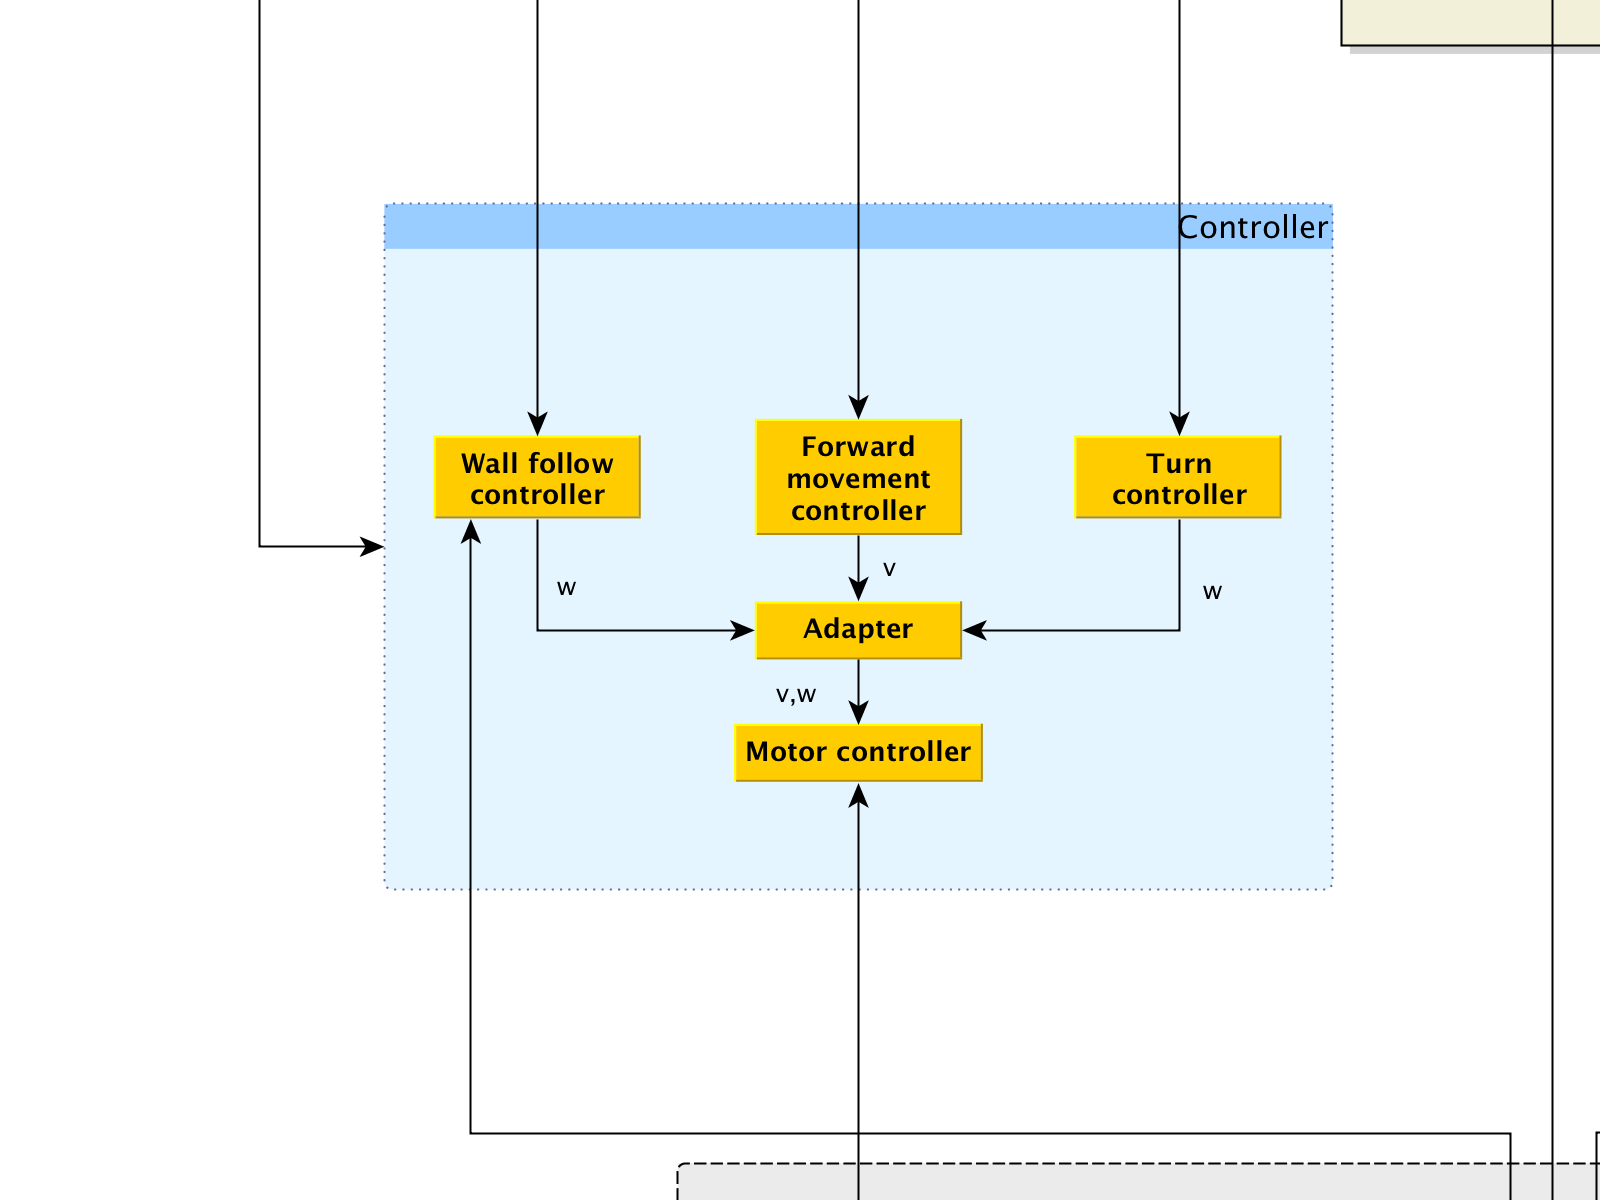
\includegraphics[width=0.6\textwidth]{figures/arch_controller.png}
\end{center}
\caption{Architecture of the controller package}
\label{fig:arch_controller}
\end{figure}

\subsection{Motor controller}

Due to internal motor difference, it is not sufficient to control the motors directly.
Otherwise the robot would move in an arch, one motor rotating slower than the other.
To compensate for that and to also be able to input linear and angular velocities, a PID controller was used. 
This enabled the robot to drive in a stable straight line.

The motors itself have a static resistance, that have to be overcome whenever the motors should transition from idling to rotating.
Overcoming these static resistance could be described by constants (for each motor one) $K_{power}$, that were added to the result of the PID results.
As soon as the static resistance has been overcome and the motor is rotating, the constant $K_{power}$ can be reduced to a value that sustains rotation: $K_{sustain}$.
This behavior results in a spiked motor control output as can be seen in figure \ref{fig:pwm_spiker}.
Although movement without spiking is possible due to the accumulating behavior of the PID controller too, it ensures responsive controlling and avoids the necessecity of increasing the gains which can easily result in overshoots.

\begin{figure}[h]
\begin{center}
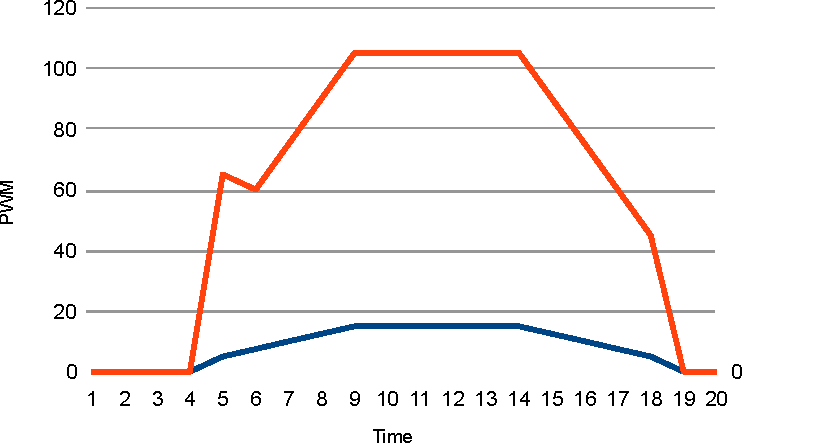
\includegraphics[width=0.6\textwidth]{figures/pwm_spike.pdf}
\end{center}
\caption{PWM Spiking for initial motor rotation attempt}
\label{fig:pwm_spiker}
\end{figure}

\subsection{Wall alignment}

The wall allignment controller (see figure \ref{fig:arch_controller}) uses the IR sensors to measure the distances from the robot to the walls, and works as follows: if both walls are close to the robot (distance < 0.4 m), then keep the robot aligned to the center between both walls.
Otherwise control only by the next closest wall, or if no wall is present, do not align.

\section*{Section Name}

Cras gravida, est vel interdum euismod, tortor mi lobortis mi, quis adipiscing elit lacus ut orci. Phasellus nec fringilla nisi, ut vestibulum neque. Aenean non risus eu nunc accumsan condimentum at sed ipsum.
\begin{wrapfigure}{l}{0.4\textwidth} % Inline image example
\begin{center}
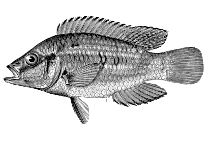
\includegraphics[width=0.38\textwidth]{fish.png}
\end{center}
\caption{Fish}
\end{wrapfigure}
Aliquam fringilla non diam sed varius. \cite{Smith:2012qr} Suspendisse tellus felis, hendrerit non bibendum ut, adipiscing vitae diam. Lorem ipsum dolor sit amet, consectetur adipiscing elit. Nulla lobortis purus eget nisl scelerisque, commodo rhoncus lacus porta. Vestibulum vitae turpis tincidunt, varius dolor in, dictum lectus. Aenean ac ornare augue, ac facilisis purus. Sed leo lorem, molestie sit amet fermentum id, suscipit ut sem. Vestibulum orci arcu, vehicula sed tortor id, ornare dapibus lorem. Praesent aliquet iaculis lacus nec fermentum. Morbi eleifend blandit dolor, pharetra hendrerit neque ornare vel. Nulla ornare, nisl eget imperdiet ornare, libero enim interdum mi, ut lobortis quam velit bibendum nibh.\cite{Smith:2013jd}

Morbi tempor congue porta. Proin semper, leo vitae faucibus dictum, metus mauris lacinia lorem, ac congue leo felis eu turpis. Sed nec nunc pellentesque, gravida eros at, porttitor ipsum. Praesent consequat urna a lacus lobortis ultrices eget ac metus. In tempus hendrerit rhoncus. Mauris dignissim turpis id sollicitudin lacinia. Praesent libero tellus, fringilla nec ullamcorper at, ultrices id nulla. Phasellus placerat a tellus a malesuada.

%------------------------------------------------

\section*{Conclusion}

Herpa derpa derp.

\begin{enumerate}
\item First numbered list item
\item Second numbered list item
\end{enumerate}

Donec luctus tincidunt mauris, non ultrices ligula aliquam id. Sed varius, magna a faucibus congue, arcu tellus pellentesque nisl, vel laoreet magna eros et magna. 

%----------------------------------------------------------------------------------------
%	BIBLIOGRAPHY
%----------------------------------------------------------------------------------------

\bibliographystyle{unsrt}

\bibliography{sample}

%----------------------------------------------------------------------------------------

\end{document}